% ------------------------------------------
%  IEEE ARTICLE TEMPLATE
% ------------------------------------------
% Author(s):
% Institution(s):
% ------------------------------------------
\documentclass[journal,twocolumn,letterpaper,10pt]{ieee-sty/IEEEtran}
\usepackage[acronym]{glossaries}
\usepackage{indentfirst}
\usepackage{url}
% Generates the acronyms list
\makeglossaries

% Acronyms list
%!TEX root = ../article.tex

% IEEE
\newacronym{IEEE}{IEEE}{Institute of Electrical and Electronics Engineers}


% ------------------------------------------
%  MAIN DOCUMENT
% ------------------------------------------
\usepackage{graphicx}
\usepackage{cite}
\usepackage{algorithm} %format of the algorithm 
\usepackage{algorithmic} %format of the algorithm 
\usepackage{multirow} %multirow for format of table 
\usepackage{amsmath} 
\usepackage{xcolor}
\usepackage{tabu} 
\begin{document}

% Variables file
%!TEX root = ./article.tex

% Article Title
%\def \ArticleTitle{A Fault Diagnosis Approach for OpenStack Considering Log Mining and Knowledg Base}

\def \ArticleTitle{A Log mining based Fault Diagnosis Framework for OpenStack Considering Knowledge Base}

% Author(s) Name(s)
\def \AuthorA{Author Name}

% Author(s) Email(s)
\def \AuthorAemail{EmailA}

% Institution(s) Name(s)
\def \InstitutionA{Tongji University}

% Article Title
\newcommand {\Title} {\ArticleTitle}

% Authors
\newcommand {\Authors} {\IEEEauthorblockN{\AuthorA}}

% Institution
\newcommand {\Institutions} {\IEEEauthorblockA{\InstitutionA}\\
                            Email: \AuthorAemail}

% Variable to control if the bibliography must be include
\def \hasBibliography{1}


% Article title
\title{\Title}

% Author(s) Name
\author{\Authors\\
        \Institutions}

\maketitle

% Abstract
%!TEX root = ../article.tex

% Abstract
\begin{abstract}
With the rapid develoment of cloud platform,the fault diagnosis for cloud platform becomes a hot research area. Although centralized management is applied for cloud platform, the size of which is still increasing, more and more components are added to the platform, which make the system difficult to diagnosis fault when fault happens. In this paper, we proposed an framework in order to facilitate the fault diagnosis of OpenStack which is currently a popular cloud platform. Fault localization techniques are used to analyse the root cause of the system failures. Event log has been widely used in fault localization techniques. Two ways are mainly adopted to localize a fault,the first is using fault model to identify a known fault;the second is using normal  behaviour model to identify the abnormal behaviour. However, due to the complexity of the cloud platform, it is still of great challenge for troubleshooting or pinpoint a fault in massive event log data.In this paper, we try to construct a log repository by collecting logs from OpenStack .During the process, some algorithms are presented for log classification, log analysis and fault log correlation analysis.
Meanwhile, we build a knowledge base repository by collecting some troubleshooting question and answers (QA) topic related to OpenStack from the famous QA websites with web crawling technology, and then propose a general automatic approach to pinpoint logs of fault from log files of open cloud platform. 
\end{abstract}

% Keywords
%!TEX root = ../article.tex

% Keywords
\begin{IEEEkeywords}
Cloud Platform,Fault Diagnosis, Log mining, ELK,Machine Learning, NLP
\end{IEEEkeywords}


% Sections

%!TEX root = ../article.tex

% Entry point for sections:
%
% This file specifies the sections and  its respective order in which they must
% be included.

% Article Sections

%!TEX root = ../article.tex

% Introduction
\section{Introduction}

Cloud Platform like OpenStack is a large complex software system. It is composed of several components and networks,it is the critical infrastructure of other software application, which means other applications should run on it. So  it already be designed with high availability and reliability in order to prevent downtime that would lead to big loss of business and revenue.When downtime occurs, the system operation administrators and the service support staff should look into the system trace and user logs to pinpoint the root cause of the failure. The straightforward process is to explore the log files manually in nature, However, a large software system normally consists of numbers modules and components in a complex environment,with each component and module writing its debug or trace log messages to a specific location, which may be a dedicated file or a database. And we fully believe that a systematic logging mechanism should be naturally built-in for a welcome software, the system logs should always reflect the running state of the software,from this point of view,there should be no exception for cloud platform. Due to the frequent interactions and high coupling,the system will generate enormous log data including at least normal information, warning information,debugging information,error information. Manually exploring millions of logs to find the root cause of a system fault is painful and inefficient. Because it is easy to image that the manual method is to search the key words in the fault information in the log data,that sound like a needle-in-a-haystack problem\cite{rao2011identifying}. \\


\setlength{\parindent}{2em}Cloud Platform like OpenStack is a cloud operating system that controls large pools of compute, storage, and networking resources throughout a datacenter, which become increasingly complex and the components within the entire system also become diverse. Once some key parts failed,the whole system would be seriously impacted due to frequent interactions. Therefore an effective fault detection and diagnosis framework can help system administrators to locate the fault and identify the root cause,which plays an critical role in large software system management. In this paper,we propose a log mining based fault diagnosis framework which is used to identify the logs which could facilitate the troubleshooting automatically via data mining from the log repository and QA knowledge base repository. We collect the logs data from the OpenStack platform, classify and analyse the logs,finally we will build a log repository, meanwhile, we try to use web crawler technology to fetch the QA topics on discussing the solution to a failure occurs in the OpenStack Platform,which usually contain a certain number of threads that users hope to provide a solution to the problem. To be briefly, in this paper,we will propose a improved classification method for fault logs,using topic clustering technology to improve the accuracy. Combining with mining the QA website,we will build a knowledge base repository to facilitate the RCA (Root Cause Analysis) process.In this Framework, the ELK (Elastic,LogStash,Kibana) Stack is adopted. LogStash is a log collector, Elastic is index database to store the log information, and the Kibana part is a real-time dashboard which is also a supplementary measure for fault diagnosis. \\

\setlength{\parindent}{2em} The remaining of this paper is organized as follows:Section II discuss the background and  related work. Section III introduce the core methodology about log mining and data prediction related to this paper. Section IV describe the overview design and implementation of the proposed framework. Section V present the experiment result and the corresponding analysis of the result. Section VI concludes with a discussion of the results. and finally is the Acknowledgement Section. 




%!TEX root = ../article.tex

% Relatedwork
\section{Related Work}
\label{related work}


\subsection{Failue detection technology in distributed system}
Paul Stelling et al.\cite{zou2014improving} proposed a fault detection service which use techniques based on unreliable fault detectors to detect and report component failure for high-performance distributed computing systems,while allowing the user to trade off timeliness of reporting against false postive.
Marin BERTIER et al.\cite{bertier2003performance}  present a failure detector implementation, in which a variant of the heartbeat failure detector, is both adaptable and designed for scalability.
Naohiro Hayashibara et al.\cite{hayashibara2002failure} identified problems for designing and implementing a scalable and generic failure detector service in a Grid system.in their paper, they describe some of the proposed protocols for failure detection and discuss their effectiveness and how they address the identified problems
Chinghway Lim et al.\cite{lim2008log} showed a approach which is to transform the chaotic log files into a standard form for visualization,Together with user feedback and simple analysis tools, visualization allowed expert knowledge to be efficiently applied to anomaly prediction, detection and
categorization.the analysis techniques in his paper led to the detection and categorization of several failure types and in some cases
predicted trends which lead towards failures.
Weiwei Shi et al.\cite{shi2016integrated} propose an improved data preprocessing framework DPF on Apache Spark for missing data prediction and fault type diagnose incorporating optimized LinR,data fusion and data cleansing to improve the quality of raw data generated by State Grid of China.
Kenji Yamanishi et al.\cite{yamanishi2005dynamic} used Syslog monitoring technologies to address a wide range of important issues including network failure symptom detection and event correlation discovery,in their paper,a new methodology of dynamic syslog mining was proposed in order to detect failure symptoms with higher confidence and to discover sequential alarm patterns among computer devices
\subsection{Fault Diagnosis related research on cloud platform}
Jia Tong et al.\cite{tong2016approach} present an approach to pinpoint bug-induced failue in logs for open cloud platforms,two algorithms called MPIN and SPIN are used in the paper to generate a predictive model based on log vectors.
Jianwen WEI et al.\cite{wei2011analysis} proposed a scalable platform for network log analysis, which targets for fast aggregation and agile query
[Cloud and Virtualization Based Log Management Service]
Sai Rakesh Ghanta et al.\cite{ghanta2017cloud} presented a solution that integrates some of the newest and popular open-source technologies, to tackle the problems that many enterprises are facing in log management
Saibharath S et al.\cite{saibharath2014design} developed a forensic framework to do cloud forensics in OpenStack for infrastructure
as a service model using the existing forensic tools
\subsection{Log mining for cloud platform}
Meera G et al.\cite{meera2016event} discusses event correlation techniques to group events logged by OpenStack tenants of interest,which ensures that the investigator views only information relevant to the tenant under suspicion
Pooya Musavi et al.\cite{Musavi2016Reliabiligy} conducted an empirical study to investigate the API failures in a cloud environment by mining bugs of 25 modules within the 5 most important OpenStack APIs.Decision Trees to build their models, but other techniques such as Support Vector Machines (SVM) and Logistics Regression should be studied and compared.
Extracting fault features with the error logs of fault injection tests has been widely studied in the area of large scale distributed systems for decades
Xiang Rao et al.\cite{rao2011identifying} present a similarity-based error log filtering method SBF to filter out noisy error logs and  increase the precision and the recall rate of fault feature extraction.
Deqing Zou et al.\cite{zou2014improving} presents a UiLog system for fault analysis and diagnosis,which collect the system log information of each component and track logs for statistics,and they proposed a Fault Keyword matrix analysis technology to classify log into different catalogues according to different fault types.
Byung Chul Tak et al.\cite{tak2016logan} presented a log analysis tool LOGAN for problem diagnosis in cloud platform,they design and develop some log correlation techniques, log comparison using templates and intuitive visualization modules.
Xiwei Xu et al.\cite{xu2014pod} we propose Process Oriented Dependability (POD)-Diagnosis, an approach that explicitly models these sporadic operations as processes. 
\subsection{ELK Stack}
ELK (Elastic Search,LogStash,Kibana) could be used as a log management system which is very convenient for user to interpret and insight the result. FigX shows the overview framework of ELK. 
Elasticsearch is a real-time distributed search and analytics engine. It allows you to explore your data at a speed and at a scale never before possible. It is used for full-text search, structured search, analytics\cite{ELKIntro2017}. Logstash is the central dataflow engine in the Elastic Stack for gathering, enriching, and unifying all of your data regardless of format or schema\cite{ELKIntro2017}.Kibana is a window into the Elastic Stack. It enables visual exploration and real-time analysis of your data in Elasticsearch\cite{ELKIntro2017}.
\begin{figure}[!h]
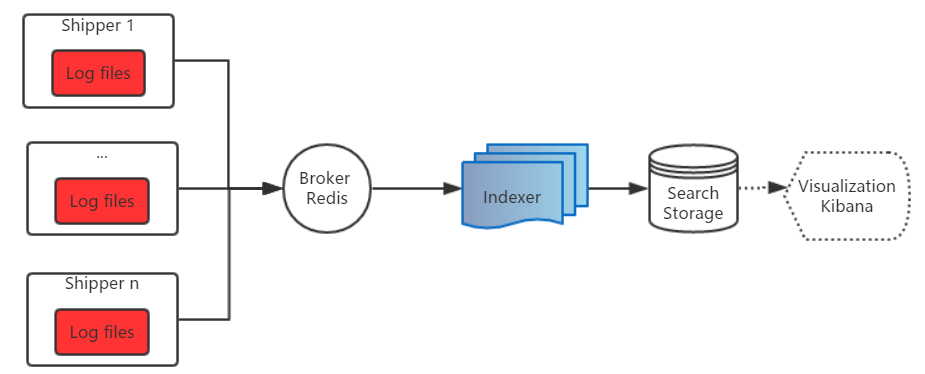
\includegraphics[scale=0.5]{./figures/Fig2.png} 
\caption{Overview of ELK Stack}
\end{figure}


%!TEX root = ../article.tex

In this section, we present the design and the implementation of the framework, the method preliminary is also presented.
\section{Data Collection and Methodology}

\subsection{Log Collection}
The logstash which is one of the key part of ELK is used as the log collector of our framework.

\subsection{QA Knowledge data Collection}

We build a web crawler framework to collect QA knowledge data from some famous QA site like StackOverflow, in which users ask and answer questions about software development,algorithms, math and other technical topics.The users participate in activities could earn users reputation by asking and answering questions. the reputation on the site is an indicator of the value of that user contribute to the site. From this point view, the answer from a user who have a good reputation on the site could be adopted by the one asking the questions. In general,when we get a troublesome issue when diagnosing the OpenStack Platform based on the error log, we could try to troubleshoot the issue via StackOverflow directly. In order to speed up the pace of troubleshooting, we build a Knowledge repository on OpenStack.Figure 3 shows a schematic the work-flow of the crawler to collect data from QA site.In this paper, we pick StackOverflow as an example to finish the experiment. \\
\begin{figure}[!h]
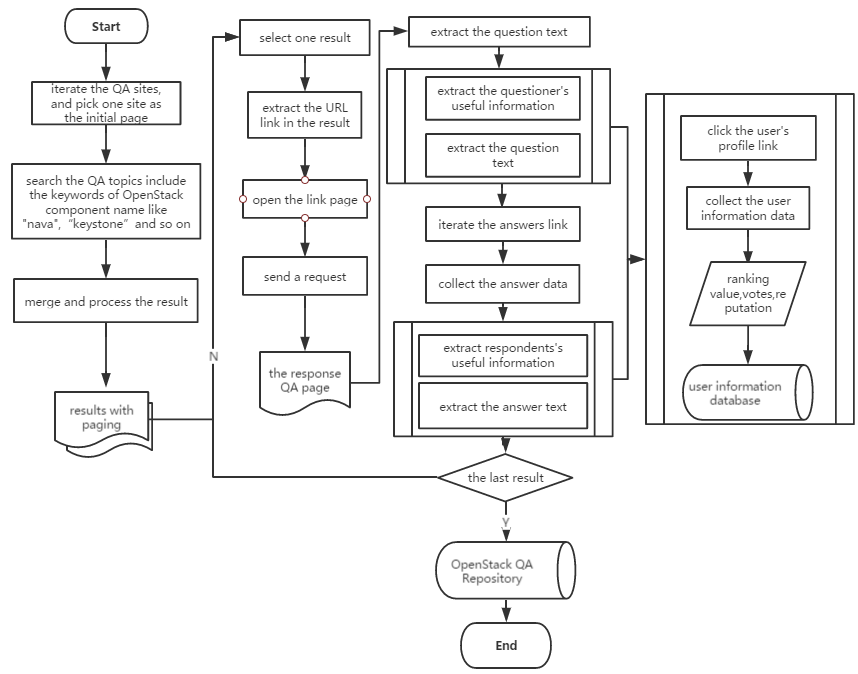
\includegraphics[scale=0.5]{./figures/Fig3.png} 
\caption{the work-flow of the crawler for collecting QA data}
\end{figure}


\renewcommand{\algorithmicrequire}{\textbf{Input:}} 
\renewcommand{\algorithmicensure}{\textbf{Output:}}

\begin{algorithm} %算法开始 
\caption{core algorithm for collecting QA data} %算法的题目 
\label{alg1} %算法的标签 
\begin{algorithmic}[1] %此处的[1]控制一下算法中的每句前面都有标号 
\REQUIRE Text:Keywords of OpenStack component,QA sites list. Variables:$list\_keywords\_openstack,list\_QA\_sites$. %输入条件(此处的REQUIRE默认关键字为Require,在上面已自定义为Input) 
\ENSURE QA information on OpenStack dataset $repo\_data$%输出结果(此处的ENSURE默认关键字为Ensure在上面已自定义为Output) 
\FOR{$site\_link$ in $list\_QA\_sites$} 

\FOR{$keyword$ in $list\_keywords\_openstack$} 
\STATE  $search\_result$ = $http\_request($$site\_link$$,$$keyword$$)$
\STATE  $search\_results.add($$search\_result$$)$
\ENDFOR

\ENDFOR

\FOR{$result$ in $search\_results$}
\STATE	$link\_topic$ = $results.link$
\STATE  {$response\_data$ = $http\_request($$link\_topic$$)$}
\STATE  {$text$ = $response\_data.question\_title$}
\STATE  $profile$ = $http\_request($$response\_data.profile\_link$$)$
\STATE  $repo\_data.add($$text$$)$
\STATE  $repo\_data.add($$profile$$)$
\STATE $answers\_results$ = $response\_data.answers$
\FOR {$answer$ in $answers\_results$}
\STATE  $answer\_text$ = $answer.content$
\STATE  $owner\_profile$ = $http\_request($$answer.owner\_link$$)$
\STATE  $repo\_data.add($$answer\_text$$)$
\STATE  $repo\_data.add($$owner\_profile$$)$
\ENDFOR
\ENDFOR
\STATE return $repo\_data$

\end{algorithmic} 
\end{algorithm}

\newcommand{\tabincell}[2]{
\begin{tabular}{@{}#1@{}}#2\end{tabular}
} 
\begin{table}[!t]  
  \centering  
  \scriptsize  
  \caption{User Schema information}  
  \begin{tabular}{ll}  
    \\[-2mm]  
    \hline  
    \hline\\[-2mm]  
    {\bf \small Key}&\qquad {\bf\small Description}\\  
    \hline  
    \vspace{1mm}\\[-3mm]  
    $id$      &   \tabincell{l}{identity of the user}\\  
    \vspace{1mm}  
    $source$          &  \tabincell{l}{source link of the source QA site}\\  
     \vspace{1mm}  
    $name$          &  \tabincell{l}{user name}\\  
     \vspace{1mm}  
    $votes$  &   \tabincell{l}{the vote count from other users from the underlying site}\\  
  	\vspace{1mm}  
    $answer\_num$  &   \tabincell{l}{the total count of answers that the user submit}\\  
     \vspace{1mm}  
    $ranking$  &   \tabincell{l}{the ranking level (percentage) in the QA site}\\  
     \vspace{1mm}  
    $top_tags$  &   \tabincell{l}{areas that the user is familiar with}\\  
     \vspace{1mm}  
    $repuataion$  &   \tabincell{l}{ reputation information}\\  
    \hline  
    \hline  
  \end{tabular}  
\end{table}  

\begin{table}[!t]  
  \centering  
  \scriptsize  
  \caption{question schema information}  
  \begin{tabular}{ll}  
    \\[-2mm]  
    \hline  
    \hline\\[-2mm]  
    {\bf \small Key}&\qquad {\bf\small Description}\\  
    \hline  
    \vspace{1mm}\\[-3mm]  
    $id$      &   \tabincell{l}{identity of the user}\\  
    \vspace{1mm}  
    $title$          &  \tabincell{l}{the title of the question}\\  
     \vspace{1mm}  
    $desc$          &  \tabincell{l}{the description/text of the question}\\  
     \vspace{1mm}  
    $votes$  &   \tabincell{l}{the vote count from other users from the underlying site}\\  
  	\vspace{1mm}  
    $tag$  &   \tabincell{l}{areas that the question belongs to}\\  
     \vspace{1mm}  
    $start\_time$  &   \tabincell{l}{the timestamp the question was created}\\  
     \vspace{1mm}   
    $update\_time$  &   \tabincell{l}{the timestamp the question was updated}\\  
      \vspace{1mm}  
    $user\_id$  &   \tabincell{l}{user id}\\  
    \hline  
    \hline  
  \end{tabular}  
\end{table} 

\begin{table}[!t]  
  \centering  
  \scriptsize  
  \caption{answer schema information}  
  \begin{tabular}{ll}  
    \\[-2mm]  
    \hline  
    \hline\\[-2mm]  
    {\bf \small Key}&\qquad {\bf\small Description}\\  
    \hline  
    \vspace{1mm}\\[-3mm]  
    $id$      &   \tabincell{l}{identity id}\\
    \vspace{1mm}  
    $user\_id$          &  \tabincell{l}{user id}\\    
    \vspace{1mm}  
    $start\_time$          &  \tabincell{l}{the timestamp the answer was created}\\  
     \vspace{1mm}  
    $update\_time$          &  \tabincell{l}{the timestamp the answer was updated}\\  
     \vspace{1mm}  
    $votes$          &  \tabincell{l}{the vote count from other users from the underlying site}\\  

    \hline  
    \hline  
  \end{tabular}  
\end{table} 


\begin{table}[!t]  
  \centering  
  \scriptsize  
  \caption{comments schema information}  
  \begin{tabular}{ll}  
    \\[-2mm]  
    \hline  
    \hline\\[-2mm]  
    {\bf \small Key}&\qquad {\bf\small Description}\\  
    \hline  
    \vspace{1mm}\\[-3mm]  
    $id$      &   \tabincell{l}{identity id}\\  
    \vspace{1mm} 
     $desc$          &  \tabincell{l}{the description/text of the answer}\\  
     \vspace{1mm}   
    $user\_id$          &  \tabincell{l}{user id}\\  
     \vspace{1mm}  
    $start\_time$          &  \tabincell{l}{the timestamp the answer was created}\\  
     \vspace{1mm}  
    $sequence$  &   \tabincell{l}{indicator of the sort order for the comments}\\  
  	\vspace{1mm}  
    $desc$  &   \tabincell{l}{the content of the comment}\\  
     \vspace{1mm}  
    $target\_type$  &   \tabincell{l}{ a label to distinguish comments for question or answer}\\  
     \vspace{1mm}  
    $target\_id$  &   \tabincell{l}{foreign key to the answer or the question}\\  
    \hline  
    \hline  
  \end{tabular}  
\end{table}

\subsection{Methodology Preliminary}
\subsubsection{Method for Data prediction}
\subsubsection{Method for Log/Topic Classification}
\subsection{Our Innovation}
In this section, we present our methodology contribution and innovation in this paper.
%!TEX root = ../article.tex

\section{The Proposed Fault Diagnosis Framework}

We will denote and introduce the proposed framework here \ldots

\subsection{Overview of the Framework}
\subsection{Building the Log Repository}
\subsubsection{Log Data Collection}
\subsubsection{Log Processing}
\subsubsection{Log Data Analysis/Root Cause Analysis}
\subsection{Building the Knowledge Base Repository}


\begin{figure}


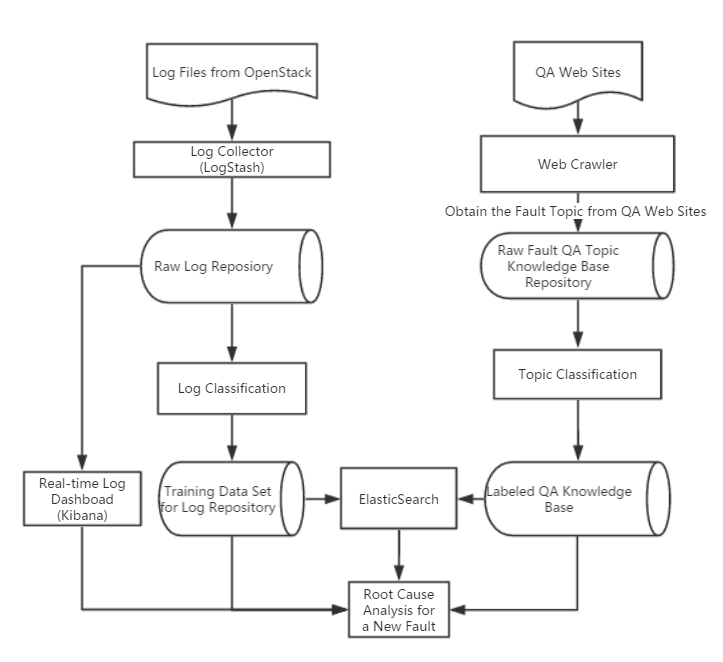
\includegraphics[scale=0.6]{./figures/Fig1.png} \label{Fig1.}
\caption{Overview framework of the proposed framework}
\end{figure}

%!TEX root = ../article.tex

\section{Expreiment and Results Analysis}

we illustrate the exprirment result in this section \\ldots
\subsection{Experimental Set Up}
\subsection{Metrics Introdcution}
\subsection{Metrics Report}
\subsection{Result Analysis}

%!TEX root = ../article.tex

% Conclusion
\section{Conclusion}

we will give a conclusion in this section \ldots


%!TEX root = ../article.tex

% Acknowledgement						
\section{Acknowledgement}
Your Acknowledgement goes here \ldots \\



\if\hasBibliography 1
% Bibliography
\bibliographystyle{IEEEtran}
% Bibliography file
\bibliography{bibliography/article}
\fi

\end{document}
